\section{PTracking}

\begin{frame}
	\frametitle{Multi-Object Detection and Tracking}
	\framesubtitle{A brief overview}
	
	\begin{columns}[t]
		\column{0.65\textwidth}
		\centering
		
		\only<1->
		{
			\vspace{0.2cm}
		}
		
		\only<1->
		{
			\begin{block}{Moving Object Detection}
				real-time extraction of moving objects from sensors
			\end{block}
		}
		
		\only<1>
		{
			\vspace{2.84cm}
		}
		
		\vspace{1.0cm}
		
		\only<2>
		{
			\begin{block}{Object Tracking\cite{Yilmaz06}}
				continuous observation of the objects over time to form persistent
				trajectories of the objects
			\end{block}
		}
		
		\column{0.3\textwidth}
		\centering
		
		\only<1->
		{
			\begin{tikzpicture}
				\node at (0,0) [draw=black,ultra thick,inner sep=0pt]  {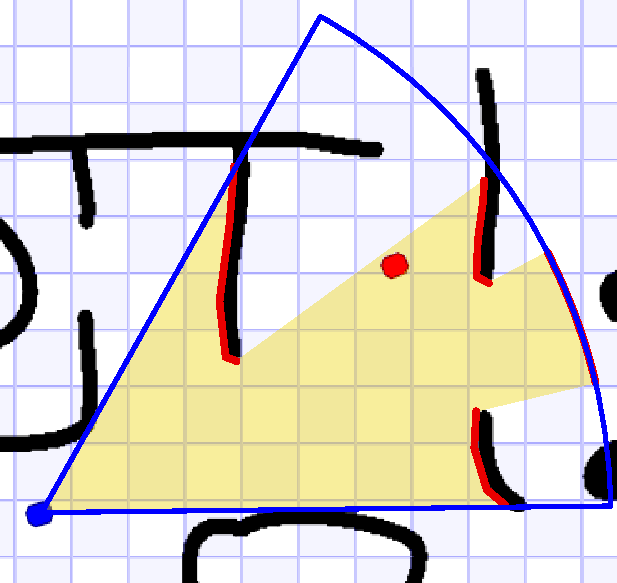
\includegraphics[scale=0.25]{Figures/Agent}};
			\end{tikzpicture}
		}
		
		\vspace{0.5cm}
		
		\only<2>
		{
			\begin{tikzpicture}
				\node at (0,0) [draw=black,ultra thick,inner sep=0pt] {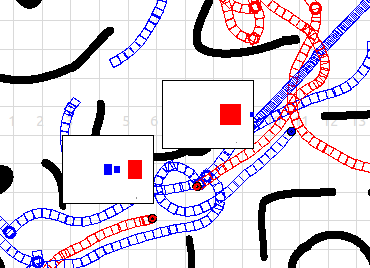
\includegraphics[scale=0.25]{Figures/Stage.png}};
			\end{tikzpicture}
		}
	\end{columns}
	
	\vspace{0.5cm}
	
	\begin{columns}
		\column{1.0\textwidth}
		
		\only<2>
		{
			\vspace{0.2cm}
		}
		
		\only<2->
		{
			\tiny 1. \emph{A. Yilmaz, O. Javed and M. Shah, ``Object tracking: A survey'' in Journal ACM Computing Surveys (CSUR), 2006}
		}
	\end{columns}
	
	\only<1>{\vspace{6cm}}
	\only<2>{\vspace{4cm}}
\end{frame}

\begin{frame}
	\frametitle{Greedy Dynamic Task Assignment (G-DTA)}
	
	\vspace{0.4cm}
	
	The G-DTA is based on the dynamic exchange of bids by predators over time. A \textbf{bid}
	is a list of costs and information gains for catching the prey.
	
	\vspace{0.4cm}
	
	\textbf{G-DTA:}
	
	\begin{enumerate}
		\item a predator creates a \textbf{new bid} each time it has seen a prey
		\item bids are \textbf{asynchronously sent} to all the predators and the G-DTA
			  algorithm makes the assignment on the basis of the current bids
		\item during the chasing, a predator \textbf{could change} the prey to chase
			  \begin{tabbing}
			  	  \hspace*{0.1cm}
			  	  
			  	  $ \leadsto $ the G-DTA algorithm assigns the prey no longer chased to\\
				  \hspace*{0.6cm}
			  	  another predator
			  \end{tabbing}
	\end{enumerate}
\end{frame}

\begin{frame}
	\frametitle{Experimental Evaluation}
	\framesubtitle{Simulation}
	
	\vspace{0.4cm}
	
	Artificial noise, calculated accordingly to the error model of real sensors, added to the
	simulated observations to better approximate a real scenario
	
	\vspace{0.2cm}
	
	\begin{table}[!t]
		\footnotesize
		
		\begin{center}
			\begin{tabular}{c c c c}
				\hline
				\textbf{Experiment} & \begin{tabular}[c]{@{}c@{}}\textbf{Prey-Predator
				Distance}\\ \textbf{(avg $ \pm $ std. dev.)}\end{tabular} &
				\textbf{Experiment} & \begin{tabular}[c]{@{}c@{}}\textbf{Prey-Predator
				Distance}\\ \textbf{(avg $ \pm $ std. dev.)}\end{tabular} \\
				\hline
				1 & 0.81 $ m $ $ \pm $ \textcolor{red}{0.13} $ m $ & 6 & 0.64 $ m $ $ \pm $
				\textcolor{red}{0.17} $ m $ \\
				2 & 1.22 $ m $ $ \pm $ \textcolor{red}{0.21} $ m $ & 7 & 0.79 $ m $ $ \pm $
				\textcolor{red}{0.31} $ m $ \\
				3 & 0.83 $ m $ $ \pm $ \textcolor{red}{0.15} $ m $ & 8 & 1.18 $ m $ $ \pm $
				\textcolor{red}{0.35} $ m $\\
				4 & 1.43 $ m $ $ \pm $ \textcolor{red}{0.08} $ m $ & 9 & 1.03 $ m $ $ \pm $
				\textcolor{red}{0.22} $ m $\\
				5 & 1.38 $ m $ $ \pm $ \textcolor{red}{0.13} $ m $ & 10 & 1.39 $ m $ $ \pm $
				\textcolor{red}{0.28} $ m $ \\
				\hline
			\end{tabular}
		\end{center}
	\end{table}
	
	\vspace{0.2cm}
	
	The \textbf{low} standard deviation demonstrates a remarkable reliability of the proposed
	approach
\end{frame}
